\section{Background of the Study}

Coffee is one of the most globally consumed beverages. It is a vital product in the global market, with production reaching 168.2 million bags in 2022-2023. The coffee industry is expected to grow even more in the coming years, with output projected to rise by 5.8\% in 2023-2024 \cite{International_Coffee_Association_2023}. In the Philippines, coffee holds a strong cultural significance, with the local industry continuously expanding. The country is the 14th largest coffee producer in the world. Locally, the industry is expected to grow at a compound annual growth rate (CAGR) of 3.5\% from 2021 to 2025, driven by small-scale farm households \cite{Santos_Baltazar_2022}. With a growing popularity among coffee enthusiasts, the demand for specialty coffee is increasing as well. Consumers are becoming more selective about the quality of their coffee beans \cite{Tampon_2023}.  

To stay competitive in the rapidly evolving coffee industry, farmers carefully select high-quality coffee beans for production. Grading green coffee beans is a crucial part of coffee production, as it is directly associated with the quality of the cup quality of coffee brews \cite{Barbosa_Scholz_Kitzberger_Benassi_2019}. Coffee grading is a process in the industry that determines the quality of coffee beans, using various parameters such as size, density, color, and defects, ensuring that only high quality beans are selected for consumption \cite{Córdoba_Moreno_Osorio_Velásquez_Fernandez-Alduenda_Ruiz-Pardo_2021}. The size of coffee beans is determined using a screen size and sorting procedure, where the coffee beans are categorized into different screen sizes, with larger beans considered higher quality \cite{González_Lopez_Taboada_Gaytán_Ramos_2019}. The density of a bean can be calculated by the ratio of its mass and volume, which greatly influences the roasting process and overall quality of the coffee \cite{Datov_Lin_2019}. Color is also another indicator for quality, with darker beans being preferred for their richer flavor profile. On the other hand, defects are classified among 3 categories: Category 1 includes the most severe issues such as foreign matter and black beans, Category 2 includes less severe defects like broken beans, and Category 3 includes minor defects like slight discoloration. Determining the quality of the coffee beans in relation to their defect values is based on quality standards and grading systems such as SCAA protocols guidance or the Philippine National Standard on Green Coffee Bean \cite{Bureau_of_Agriculture_and_Fisheries_Standards_2012}. 

Traditionally, this stage of assessing and categorizing coffee beans relies on visual evaluation, which is time-consuming and labor-intensive, making it prone to human error. One of the biggest challenges in coffee bean production is ensuring consistency in quality. As the demand for specialty coffee continues to grow, there has also been an increase for the need of more efficient and accurate sorting methods. The application of modern technology can help reduce the labor costs and minimize human errors in these tasks. In recent years, computer vision was used alongside various machine learning models and techniques, such as convolutional neural networks (CNNs), support vector machines (SVMs), or K-nearest neighors (KNN) models, where the models were trained on labeled data to classify images of coffee beans into different quality categories. The proposed study aims to utilize this technology to develop a two-stage automated coffee bean sorting system using machine vision and density-based analysis to categorize and identify defects, good beans, dense, and less-dense green coffee beans. 

\section{Prior Studies}
Identifying and sorting specialty-grade coffee beans can be strenuous since the traditional way of classifying a specialty-grade coffee is by manually sorting the coffee bean batch and classifying them according to the set of standards of the SCAA. The existing work aims to solve these problems through image processing and implementing deep learning-based models to automatically sort the coffee beans while achieving high accuracy. However, these solutions only automate detecting either one of the parameters such as defects, color, and size, while the proposed system considers density, color and defects all in one system. Hence, eliminating human intervention or labor. The table below shows the comparison of existing solutions to the researcher’s proposal aligning with the traditional way of sorting coffee beans.

\begin{center}
    \begin{longtable}{| p{4cm} | p{10cm} |}
	\caption{Summary of the Literature Review}
	\label{summary_literature_review}
	\endfirsthead
	\endhead
    \hline
    Existing Literature & Description \\ \hline
    Defect Detection & The existing literature focuses on using various machine learning models such as YOLO, KNN, and CNN to detect defects in green coffee beans, 
	through identifying visible defects like black spots, broken beans, discoloration, and more. These existing approaches heavily rely on visual characteristics 
	and do not consider other key factors that affect green coffee bean quality like density, which can enhance classification accuracy. The proposed system 
	integrates density and size analysis alongside the defecting various levels of defects on the coffee bean for a more holistic detection and classification. \\ \hline
    Coffee Bean Grading and Quality Assessment & The existing literature utilize algorithms such as artificial neural networks, support vector machine, and random 
	forest to grade and classify coffee beans according to the specified grading system. These methods primarily focus on visual features of the beans, 
	which do not account the bean’s density and size, which are both essential factors for classifying specialty-grade coffee beans. Additionally, there is a lack of 
	practical implementation of automated sorting systems, as these focus on simply classifying the beans. Through a two-stage process, the proposed system will 
	take into consideration both the visual inspection and the density measurement, which leads to a more complete classification of coffee beans. \\ \hline
    Automated Sorting and Classification System & Research has been conducted on developing that automate the process of sorting coffee beans according to various parameters. 
	Some studies focus on sorting defectives against non-defective, while others focus on other visual parameters like defects and roast profiles. These systems focus only on visual 
	characteristics, without considering the actual size of the bean and its density as parameters for better classification accuracy. The proposed system will integrate the use of visual, density, and size parameters to enable a comprehensive automated sorting solution for classifying specialty-grade coffee beans. \\
    \hline
    \end{longtable}
\end{center}

\begin{center}
	\scriptsize{
    \begin{longtable}{| p{0.3\textwidth} | p{0.3\textwidth} | p{0.3\textwidth} |}
	\caption{Comparison Table on Existing Studies} 	
	\label{comparison_table_existing_studies}
	\endfirsthead
	\endhead
    \hline
    Proposed System & \cite{Balay_Cabrera_Jensen_Mayuga_2024} & \cite{Lualhati_Mariano_Torres_Fenol_2022}\\ \hline
    
	\begin{itemize}
		\item Defect sorting using RFDETR, YOLOv12, and Vision Transformer models. 

		\item Considers classification of 7 defect types. 
	
		\item The system considers density parameters to sort out less-dense beans. 
	
		\item The system includes a graphical user interface for farmers to visualize the cumulative data of the defects present in the batch. 
	
		\item The system also includes AI-generated recommendations on the possible interventions for the farmers based on the data gathered from the sorting system.  
	\end{itemize}
	&
	\begin{itemize}
		\item Defect sorting using YOLOv8 

		\item The study considered only 6 types of defects. 
	\end{itemize}
	&
	\begin{itemize}
		\item Defect sorting using YOLOv2 and InceptionV3. 
		\item The study considered only 2 types of defects. 
	\end{itemize}
	\\
	\hline
    \end{longtable}
	}
\end{center}

\section{Problem Statement}
The Philippine coffee industry is a growing market, however it is stuck with using traditional methods in sorting green coffee beans. Often relying on manually sorting the beans, it exposes a number of problems that are apparent in the industry. Relying on manual sorting increases production cost which results in higher prices for quality coffee beans. To make the Philippine coffee beans more competitive to the exported beans, reducing the price is crucial. Another problem that is encountered in manual sorting heavily focuses only on the physical attributes of the bean like size and appearance. There are standards that need to be met, which forces the farmers to resort to manual sorting to comply with the standards of the SCAA. The SCAA standards require a 300g batch of green coffee beans must not contain any defects and the size consistency of the beans must not exceed 5\% variance. Another reason why coffee processors still opt to do manual sorting is because there are no commercially available and reliable GCB sorting machines \cite{Lualhati_Mariano_Torres_Fenol_2022}. There is a need for a coffee sorter that is able to efficiently and accurately sort GCB. Coffee bean selection is carried out either manually, which is a costly and unreliable process \cite{Santos_Rosas_Martins_Araújo_Viana_Gonçalves_2020}. The manual sorting process limits scalability and quality control, putting the strain on farmers as coffee shop owners' demands for high-quality coffee continue to rise \cite{Lualhati_Mariano_Torres_Fenol_2022}.   	 	 

\section{Objectives and Deliverables}

% TODO: UPDATE BASED ON NEW OBJECTIVES
\subsection{General Objective (GO)}
 \Copy{GO}{GO: The study aims to develop an automated (Arabica) green coffee bean sorter that identifies good, less-dense and defective beans from an unsorted batch of coffee beans. The system will utilize machine vision and density-based analysis for defect detection and classification of the coffee beans, ensuring efficient coffee bean sorting.};

\subsection{Specific Objectives (SOs)}

\begin{itemize}
	\item \Copy{SO1}{SO1: To gather and create a dataset consisting of 500 high-resolution images of good Arabica green coffee beans and 200 high-resolution images per classification of defective beans (Category 1 \& Category 2).};
	
	\item \Copy{SO2}{SO2: To improve the synchronization between the machine vision system and the embedded sorting mechanism, ensuring defect sorting of at least 20 beans per minute for stage one, solving issues such as non-synchronization of the system.};
	
	\item \Copy{SO3}{SO3: To achieve an accuracy of at least 85\% in classifying defective green coffee beans using computer vision};
	
	\item \Copy{SO4}{SO4: To achieve an accuracy of at least 85\% in filtering out less-dense green coffee beans};
\end{itemize}

\subsection{Expected Deliverables}

Table ~\ref{tab:expected_deliverables} shows the outputs, products, results, achievements, gains, realizations, and/or
yields of the \documentType. 


\begin{table}[H]
	\caption{Expected Deliverables per Objective} 	
	\label{tab:expected_deliverables} 
	{\centering \scriptsize
		\begin{tabular}{p{0.2\textwidth}|p{0.7\textwidth}}
			\hline 
			\hline 
			\textbf{Objectives} & 
			\textbf{Expected Deliverables}\\ 
			\hline 
%%			\endfirsthead
%			\multicolumn{2}{c}%
%			{\textit{Continued from previous page}} \\
%			\hline
%			\hline 
%			\textbf{Objectives} & 
%			\textbf{Expected Deliverables}\\ 
%			\hline 
%%			\endhead
%			\hline 
%			\multicolumn{2}{r}{\textit{Continued on next page}} \\ 
%%			\endfoot
%			\hline 
%%			\endlastfoot
%			\hline							

			\Paste{GO} & A Two-Stage Automated Coffee Bean Sorter System that identifies defective, good beans, and less-dense green coffee bean using machine vision and density-based analysis.  \\ \hline

			\Paste{SO1} & \begin{itemize}
				\item Data Gathering 

				\item Image Collection through High Quality Camera 
			\end{itemize} 
			\\ \hline		
%
			\Paste{SO2} & \begin{itemize}
				\item Improving the synchronization of machine vision and embedded sorting mechanism of the system.
			\end{itemize} 
			\\ \hline
%						
			\Paste{SO3} & \begin{itemize}
				\item Computer Vision Program 
				\item Sorting Mechanism 
			\end{itemize} 
			\\ \hline
%						
			\Paste{SO4} & \begin{itemize}
				\item Density-based Analysis 
				\item Sorting Mechanism 
			\end{itemize} 
		 	\\ \hline
		\end{tabular}
	}
\end{table}



\section{Significance of the Study}

The study explores the implementation of machine vision and density analysis of an automated coffee been sorter that can identify and sort out the defective, less-dense and good green coffee beans. This said system would aid coffee sorters to mitigate manual labor and to ensure that the sorting process of the GCB are accurate. In order to test the effectiveness of the system, the study would gather data and compare the time efficiency and accuracy of the manual sorting by a an expert sorter to be compared with the proposed system. The system proposes significance to specific parts of society as follows: 

\subsection{Technical Benefit}

This study would benefit the academe as this introduces a significant advancement in coffee bean sorting technology by implementing both machine vision and density-based analysis to detect and sort good coffee beans, less-dense and separating defective ones. The proposed system would mitigate manual sorting that leads into insufficency like human error and fatigue. The system would improve the overall efficiency by operating at a faster rate compared to manual labor. As a result, it would serve as a proof of concept for the implementation of machine vision and  density-based analysis in agricultural  industries specifically in the Philippine coffee industry. 

\subsection{Impact to the Coffee Industry}

The study would aid coffee farmers and producers, by providing an automated system that ensures accurate sorting of Arabica green coffee beans, the system aims to have an accurate output to help maintain to yield higher quality coffee beans and allows coffee bussinesses to scale up their operations, increase the competitiveness of  exporting those beans, and meet demand more efficiently. The productivity given from the system would potentially strengthen the foundation of local coffee producers.  

\section{Assumptions, Scope, and Delimitations}

\subsection{Assumptions}

\begin{enumerate}
	\item There would be a defective coffee bean from the green coffee bean test batch;
	
	\item Identifying the defective coffee beans using the machine vision and density-based analysis would be much more efficient and accurate than manually sorting them;
	
	\item During testing, test batches will contain 50\% good beans and 50\% defective beans, 75\% good beans and 25\% defective beans, 25\% good beans and 75\% defective beans, 100\% defective beans, and 100\% good beans;	
\end{enumerate}

\subsection{Scope}
\begin{enumerate}
	\item The study only focuses on Arabica green coffee beans;
	
	\item The study has two stages, the first stage would segregate the defective green coffee beans from the batch, then the second stage would identify the specialty-grade green coffee beans depending on its density;

	\item The study will only consider the following metrics for classification: Color, Shape, Physical Characteristics, Density, and Texture.

	\item The system is not designed to evaluate other coffee bean varieties or factors such as moisture content, different coffee bean origins, bean size beyond the allowed deviation, or post-roasting characteristics.

\end{enumerate}

\subsection{Delimitations}
\begin{enumerate}
	\item The batch of coffee beans to be used for testing and dataset collection will consist solely of Arabica beans from the same origin, farmer, and processed in the same way;
	
	\item The system is only limited to unroasted green coffee beans;
	
	\item The batch of coffee beans to be used should only be dehulled and not sorted visually and by density;

	\item Since the system is considering several types of defects and density parameter, sorting time is compromised;

	\item The system is designed to perform individual scanning of each coffee bean;

	\item Sizing will not be considered, as it may cause jamming in the system. However, a maximum size deviation of 20\% among beans will be allowed.

	\item This study is limited to detecting only the most evident defect in a green coffee bean when multiple defects are present. The system prioritizes the most prominent defect based on visual characteristics and does not classify multiple defects per bean.

\end{enumerate}

\subsection{Overview of the Methodology}

The rapid advancements in computer engineering have led to innovative solutions across various domains, including artificial intelligence and embedded systems. This thesis presents a novel approach to automated coffee bean sorting, addressing key challenges in manual classification and proposing a two-stage system that integrates machine vision and density-based analysis.

The study explores fundamental principles and technologies relevant to coffee bean classification, including machine vision, deep learning, and density-based sorting. By combining theoretical analysis with practical implementation, the proposed system aims to enhance sorting accuracy, reduce human labor, and improve efficiency and quality output in coffee production. 

The study’s objective is to create a dataset consisting of 500 high-resolution images of Arabica specialty-grade green coffee beans from a certain origin, to ensure sufficient data for training and validation of the algorithm in the machine vision system. The system will capture real-time data on the visual and density characteristics of each green coffee beans, to aid coffee farmers from sorting each coffee bean efficiently. In the succeeding chapters, the study will delve into existing research on automated coffee bean sorting systems, with a focus on machine vision, density analysis, and their applications in the coffee industry. The study would explore gaps in current manual sorting practices and demonstrate the system’s ability to improve overall efficiency through implementing advanced technologies.

\subsection{Estimated Work Schedule \& Budget}

\begin{table}[H]
    \centering
    \caption{Budget Plan}
    \label{tab:budget_plan}
    \resizebox{\textwidth}{!}{%
    \begin{tabular}{l c c r}
    \toprule
    \textbf{Item} & \textbf{Quantity} & \textbf{Price} & \textbf{Total} \\
    \midrule
    IP Camera                                     & 2          & 999   & 1,998 \\
    Arduino Nano                                 & 2          & 300   & 600   \\
    ToF10120                                     & 1          & 400   & 400   \\
    Acrylic Platform                             & 1          & 67    & 67    \\
    12 NEMA Stepper Motor                        & 1          & 405   & 405   \\
    6V DC Motor                                  & 1          & 150   & 150   \\
    TB6612FNG Motor Driver                       & 1          & 50    & 50    \\
    MT3608 Step-Up Module                        & 1          & 50    & 50    \\
    Lighting Equipment (LED Bar, Ring, Spotlight)& 3          & 80    & 240   \\
    Precision Weighing Scale                     & 1          & 2,000 & 2,000 \\
    HX711                                        & 1          & 69    & 69    \\
    Rotating Conveyor Table 3D Printing          & 1          & 5,000 & 5,000 \\
    Inspection Tray 3D Printing                  & 1          & 4,700 & 4,700 \\
    Density Sorter 3D Printing                   & 1          & 2,500 & 2,500 \\
    Screw Feeder 3D Printing                     & 1          & 3,500 & 3,500 \\
    \textit{Other Hardware Components/Wires}     & \textit{Approximate} & \textit{Approximate} & \textit{Approximate} \\
    \midrule
    \textbf{Total Estimate}                      &            &       & \textbf{21,879 + approximate additional hardware components} \\
    \bottomrule
    \end{tabular}%
    }
\end{table}

\begin{figure}[H]
    \centering
    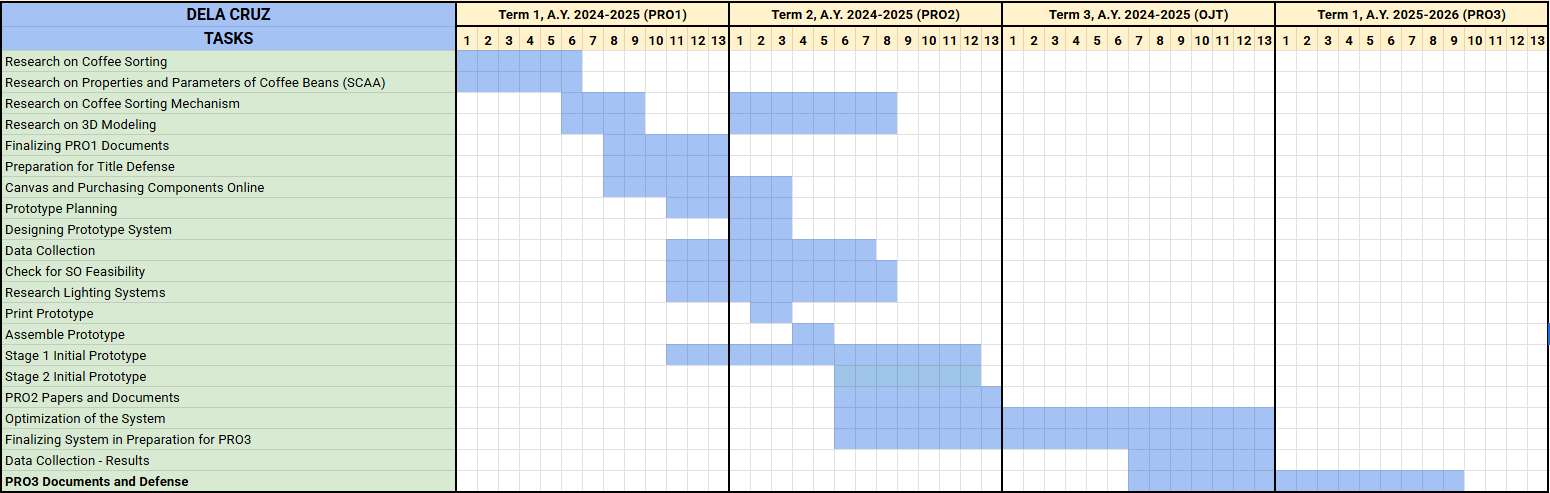
\includegraphics[width=\textwidth]{ch1/GanttChart_DelaCruz.png}
    \caption{Gantt Chart for John Carlo Dela Cruz}
    \label{fig:gantt_jc}
\end{figure}
\begin{figure}[H]
    \centering
    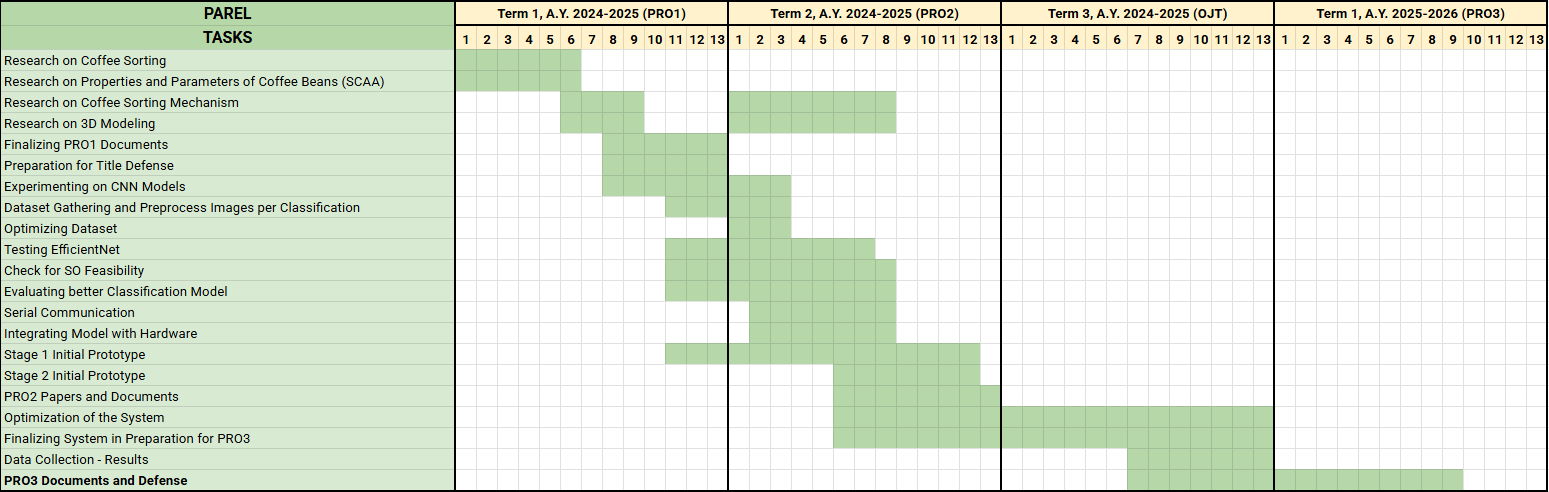
\includegraphics[width=\textwidth]{ch1/GanttChart_Parel.png}
    \caption{Gantt Chart for Pierre Parel}
    \label{fig:gantt_pierre}
\end{figure}
\begin{figure}[H]
    \centering
    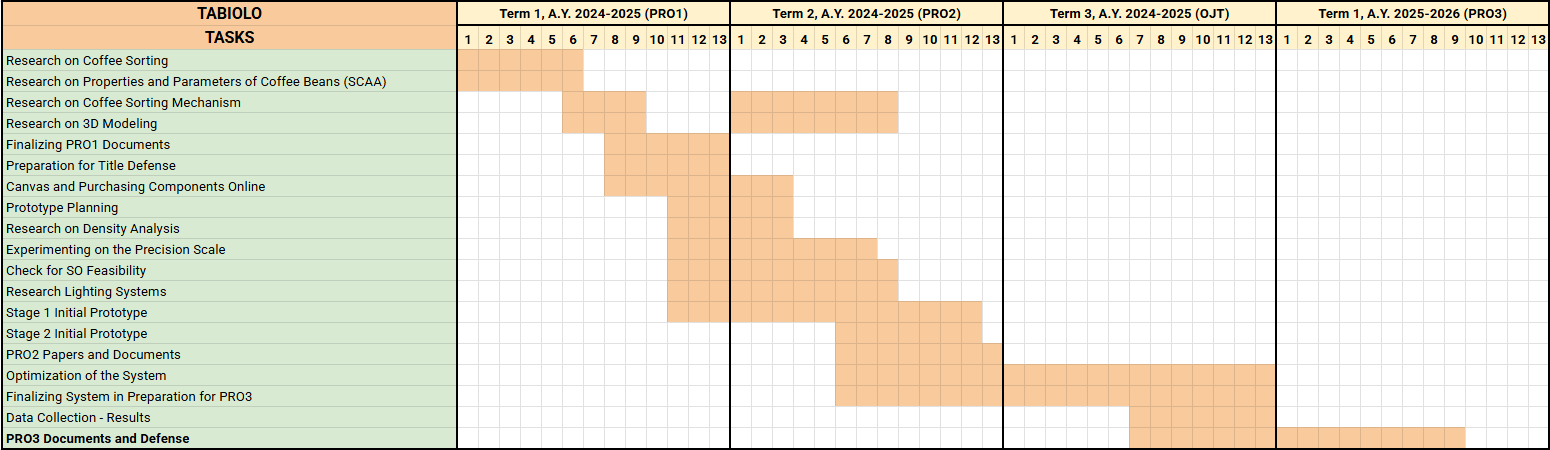
\includegraphics[width=\textwidth]{ch1/GanttChart_Tabiolo.png}
    \caption{Gantt Chart for Jiro Tabiolo}
    \label{fig:gantt_jiro}
\end{figure}
\begin{figure}[H]
    \centering
    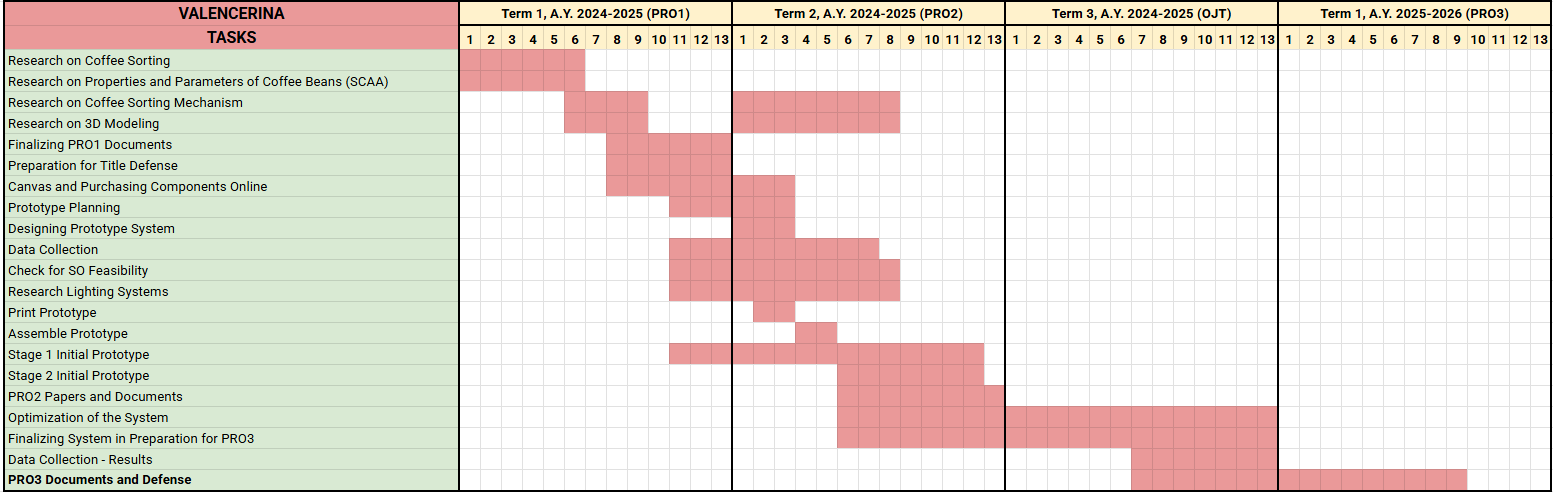
\includegraphics[width=\textwidth]{ch1/GanttChart_Valencerina.png}
    \caption{Gantt Chart for Ercid Bon Valencerina}
    \label{fig:gantt_bon}
\end{figure}